\section{Assignment 1}
\subsection{Introduction and objectives}
This assignment implements a numerical simulator for a damped wave
propagating across a two-dimensional domain, governed by the partial
differential equation:
\begin{equation}
    \frac{\partial^{2}u}{\partial t^{2}}+\gamma\frac{\partial u}{\partial t}=c^{2}\nabla^{2}u
\end{equation}
Physically, this couples wave propagation (the $c^{2}\nabla^{2}u$ term,
which spreads a local disturbance outward at speed $c$) with viscous
damping (the $\gamma\,\partial u/\partial t$ term, which dissipates
energy over time and drives the field back toward rest); $u(x,y,t)$ is
the wave's height at position $(x,y)$ and time $t$. Beyond producing a
visual MP4 of the simulation, this first assignment's real purpose is to
establish the OpenMP-parallelized simulation core that Assignments 2 and
3 build on directly: the same discretization, the same stencil update,
and the same per-frame output pattern reappear largely unchanged in the
later multi-rank and GPU-accelerated versions.

\subsection{Implementation}
The continuous model is discretised on a regular grid: space is divided
into points spaced by $\Delta x$ and $\Delta y$, and time into steps of
$\Delta t$. Each grid point is identified by indices $(i,j)$ and each
instant by an index $t$, so that $u(x,y,t)$ becomes a matrix of values
$u_{i,j}^{t}$. The derivatives in the equation are approximated with \textbf{central differences method} \cite{finitedifference}, so that the next wave state $u_{i,j}^{t+1}$ is:
\begin{equation}
    \resizebox{0.9\textwidth}{!}{$
        u_{i,j}^{t+1} = \frac{1}{\gamma \Delta t + 2} \left[ c^2 \Delta t^2 \left( \frac{u_{i+1,j}^t - 2u_{i,j}^t + u_{i-1,j}^t}{\Delta x^2} + \frac{u_{i,j+1}^t - 2u_{i,j}^t + u_{i,j-1}^t}{\Delta x^2} \right) + \gamma u_{i,j}^{t-1} \Delta t - 2u_{i,j}^{t-1} + 4u_{i,j}^t \right]
    $}
\end{equation}
The temporal evolution is handled with three $M \times M$ matrices,
\texttt{u\_past}, \texttt{u} and \texttt{u\_fut}, dynamically allocated
with \texttt{malloc} and representing the wave state at times $t-1$, $t$
and $t+1$ respectively. All elements are initialised to zero except for a
single impulse at the centre of the grid $(M/2, M/2)$, used to start the
perturbation.

The core of this assignment is the parallelization of the update loop
with \textbf{OpenMP}. A \texttt{\#pragma omp parallel} region is opened
once before the time loop, and the two nested spatial loops are
distributed across threads with \texttt{\#pragma omp for
schedule(static) collapse(2)}: \texttt{schedule(static)} splits the
iterations into equal-sized chunks assigned before execution \cite{slidestatic}, while
\texttt{collapse(2)} fuses the $i$ and $j$ loops into a single
$M\times M$ iteration space \cite{openmpcollapse}, giving the scheduler far more, finer-grained
work units to balance across cores. Each thread thus computes
$u_{i,j}^{t+1}$ for a disjoint set of coordinates, independently and
concurrently with the others.

Once \texttt{u\_fut} has been fully computed for the current timestep, it
must be written to a PGM file; this is done inside a \texttt{\#pragma omp
single} block, so that only one thread performs the write while the rest
wait at the implicit barrier. To avoid the cost of deep-copying entire
matrices between timesteps, the temporal advance is implemented as a
three-way pointer rotation (\texttt{u\_past} takes the address of
\texttt{u}, \texttt{u} takes that of \texttt{u\_fut}, and \texttt{u\_fut}
is recycled for the next iteration), performed by the same thread that
just wrote the file. This keeps the pointer swap race-free and avoids any
extra synchronization beyond the barrier already required for the write.

\subsubsection{Identified inefficiencies and corrective transformations}
All profiling and testing in this section was performed using the \texttt{Edu\_skylake} partition (4 nodes, 32 physical and logical cores) \cite{hpcguide} with 32 threads
and a workload size of $M = 1000$. The aim was to identify the main bottlenecks and improve the source code.

We profiled the initial implementation with \textbf{Intel VTune
Profiler}. \textit{Hotspots} analysis identifies which functions in an
application consume the largest share of execution time, using
low-overhead sampling to build a ranked list of hotspot functions as a
starting point for optimization \cite{vtune-hotspots}. \textit{Threading}
analysis instead evaluates how efficiently the application uses the
available processor cores, exposing inefficiencies in threading-runtime
usage and contention at synchronization points that leave threads idle
and prevent full processor utilization, summarized through its
\textit{Effective CPU Utilization} metric \cite{vtune-threading}.
Combining the two analyses lets us separate genuine computation time from
time lost to idle spinning at synchronization points.

Hotspot analysis showed that \texttt{gomp\_team\_barrier\_wait\_end} and
\texttt{fwrite} accounted for 79.4\% and 9.7\% of total CPU time
respectively, against only 2.2\% for the matrix computation itself: the
bottleneck was therefore not the stencil, but excessive synchronization
and I/O overhead. Three successive transformations addressed this, each
verified either via VTune or direct code inspection.

Three successive transformations addressed this, each verified either
via VTune or direct code inspection. Frames were originally written
pixel by pixel with \texttt{fwrite()} inside a single-threaded
\texttt{\#pragma omp single} block; replacing this with an in-memory
buffer, filled in parallel via a dedicated \texttt{\#pragma omp for} and
flushed to disk with one \texttt{fwrite()} call, cut I/O calls from one
per pixel to one per frame, though it introduced a new barrier, since the
buffer-fill loop was a separate worksharing construct from the stencil
loop. Since the stencil and the buffer-fill iterate over the exact same
$(i,j)$ range, however, we then merged them into a single
\texttt{\#pragma omp for}, writing each scaled pixel immediately after
computing \texttt{u\_fut[i][j]} and removing that extra barrier again
with no loss of parallel work. Finally, the matrix initialization,
originally performed sequentially by a single thread, was parallelized
with \texttt{\#pragma omp parallel for}. By
Amdahl's law, this serial fraction would otherwise cap the achievable
speedup regardless of how well the main loop scales. On a multi-socket
compute node, each CPU socket has its own directly-attached memory
bank: cores access memory local to their own socket faster than memory
attached to another socket, a design known as NUMA (Non-Uniform Memory
Access) \cite{numaslides}. Under the default \textit{first-touch} policy, a physical page
is assigned to the socket of whichever thread writes to it first, we therefore gave
the initialization loop the same schedule as the stencil loop, so that
each thread's first-touch region matches the region it repeatedly
accesses afterwards. Profiling the complete pipeline
(including I/O) showed, however, that \texttt{schedule(guided)}
outperforms \texttt{schedule(static)} in practice \cite{output_guided_static_m1000}:
under \texttt{guided} scheduling,
chunks are handed out to threads on request rather than fixed in advance,
with each chunk's size proportional to the number of remaining
iterations and shrinking toward the specified minimum (1 as default) as the loop
progresses \cite{openmpcollapse}.This dynamic redistribution better
compensates for the load imbalance introduced by the single-threaded
frame-writing step, so \texttt{guided} was retained for the final
implementation. As shown later in the testing section,
isolating the computation from I/O reverses this result, confirming that
NUMA locality does matter once the synchronization overhead of I/O is
removed.

After these three improvements, VTune Hotspot analysis showed a clear
shift in where CPU time was spent: \texttt{gomp\_team\_barrier\_wait\_end}
fell from 79.4\% to 57.5\%, the matrix computation itself rose from
2.2\% to 15.7\%, and I/O (\texttt{fwrite}) time dropped from 9.7\% to
under 0.3\% \cite{output_after_improvements}. The Threading analysis, however,
revealed that the program was still using only 23\% of the available
CPUs, for an average effective utilization of 7.362 out of 32 threads:
a clear sign that, at $M=1000$, the workload was simply too small for the
number of threads requested. This motivated the next round of tests,
which vary the workload size and other parameters to see how resource
utilization changes.

\subsection{Testing and Results}
\label{sec:testing}
Having used \texttt{edu\_skylake} purely to identify and fix code-level
bottlenecks, the remaining tests moved to a larger, more capable
partition to study the HPC system's own architectural behavior under
realistic workloads -- NUMA effects, Hyper-Threading, and multi-node
scaling -- rather than the code itself. The remaining tests were run on the \texttt{Edu\_sapphire} partition
(2 nodes, 48 physical and 96 logical cores each); each node is dual-socket,
with 24 physical cores per socket \cite{hpcguide}.
\subsubsection{Sweep of workload size}
\begin{figure}[h]
    \centering
    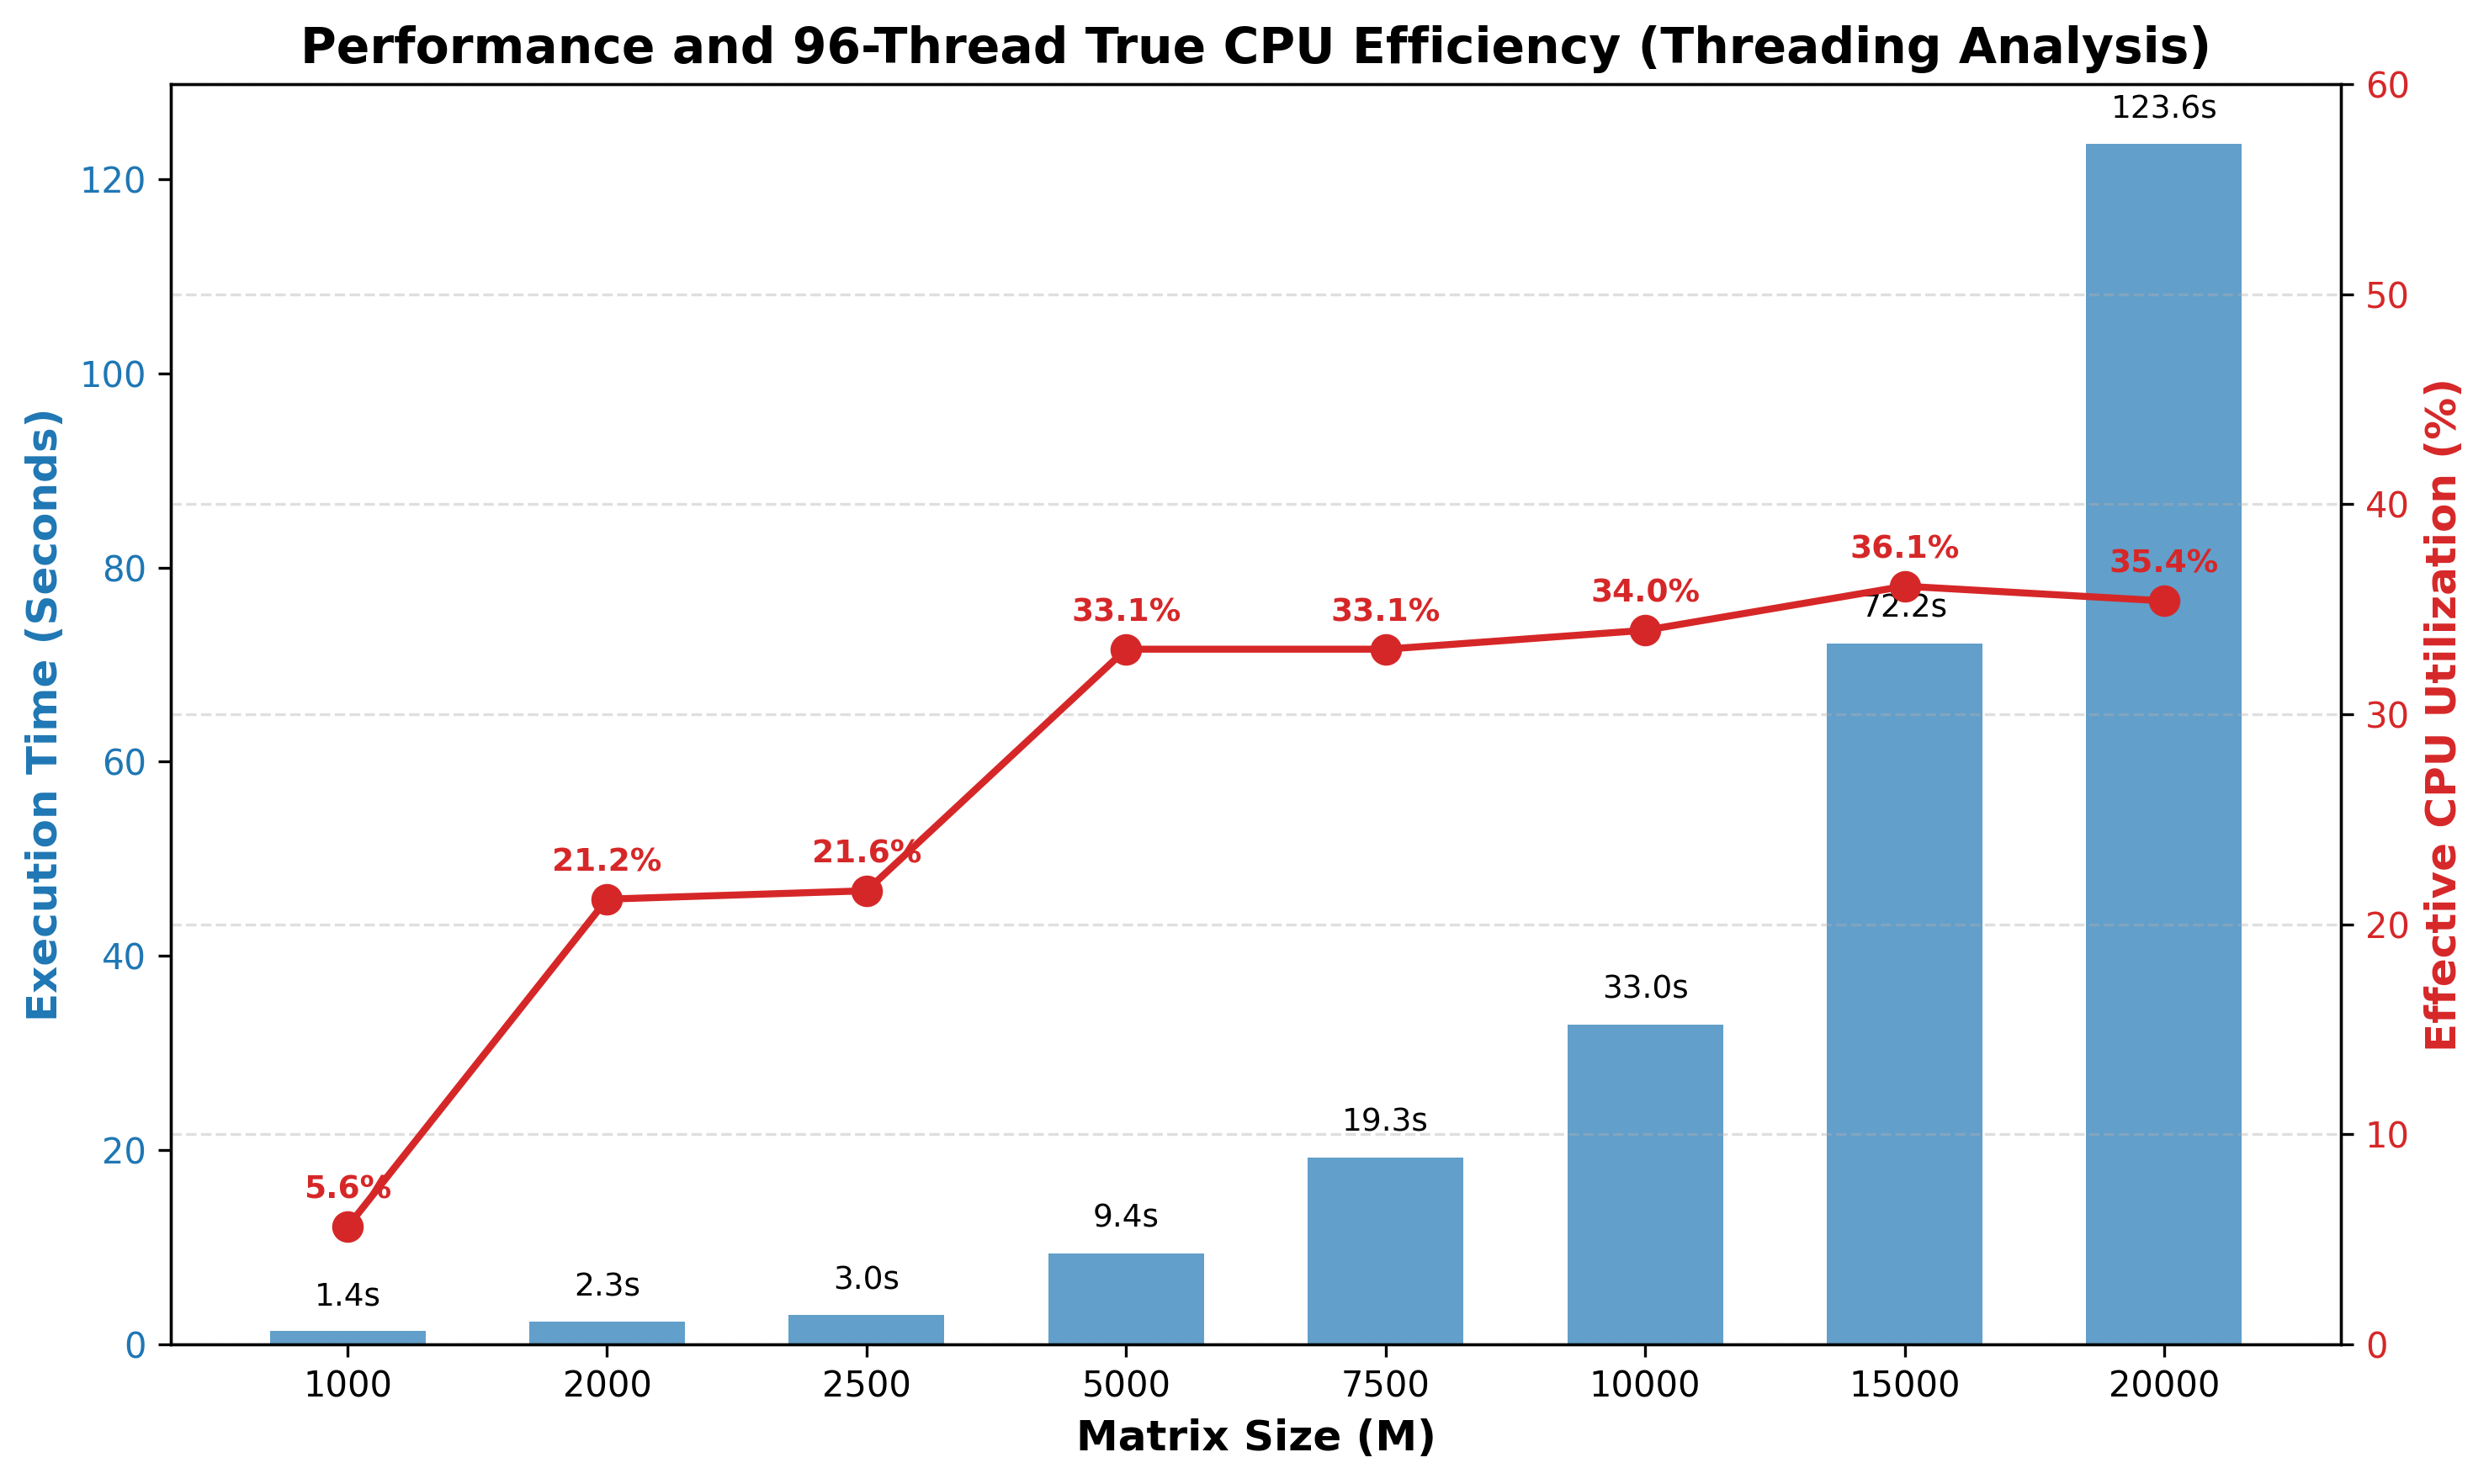
\includegraphics[width=0.46\textwidth]{../assignment_1/plots/timeandCPUU96.png}
    \caption{Execution time and true CPU efficiency scaling with varying grid sizes ($M$), using 96 threads.}
    \label{fig:performance_scaling}
\end{figure}

In order to investigate the architectural limits of the system, a workload sweep test was conducted using the maximum logical capacity of the compute node (96 threads), varying the grid size $M$ from 1,000 to 20,000. Figure \ref{fig:performance_scaling} illustrates the execution time (extracted without the profiling overhead)vs the True Effective CPU Utilization, extracted from the VTune threading analysis.
The utilization curve reveals three distinct operational phases. For small grids ($M=1000$ to $2500$), the system suffers from severe \textit{thread starvation}, 
where the computational workload is too small to justify the distribution across 96 threads and two NUMA sockets, resulting in an initial efficiency plateau around 21\%, dominated by synchronization overhead, barrier wait times and I/O operations.
As $M$ increases ($M=5000$ to $15000$), the computational density grows quadratically ($O(M^2)$) the useful computational work begins to outweigh the fixed parallelization overhead, driving the CPU utilization upward.\\
However, the efficiency strictly plateaus at approximately 36\% for massive grids ($M \ge 15000$). This hard limit is the superposition of three architectural constraints: 
the strict sequential bottleneck of the disk I/O operations (Amdahl's Law), the saturation of the memory bandwidth (memory wall), and the effects of Hyper-Threading. Regarding the latter, since the node possesses only 48 physical cores, through Hyper-Threading each core exposes two logical processors to the OS, which share the same exectuion units, caches and memory bandwidth \cite{marr2002hyperthreading}. So, attempting to utilize 96 threads for a memory-bound stencil operation forces logical threads to heavily compete for the same physical cache resources, preventing the utilization from approaching 100\%.
Regarding the absolute execution times, the data perfectly validates the theoretical $O(M^2)$ spatial complexity of the 2D grid simulation. For instance, doubling the grid dimension from $M=10000$ to $M=20000$ effectively quadruples the computational domain and the execution time scales from 33.0 seconds to 123.6 seconds, achieving a 3.74x increase that is remarkably close to the theoretical 4x factor. Conversely, in the smaller grid range ($M \le 2500$), the constant overhead associated with managing 96 concurrent threads, along with the fixed costs of implicit OpenMP barriers, heavily dominates the actual execution time, confirming the thread starvation phenomenon observed in the efficiency curve.
\subsubsection{Sweep of number of threads at $M=15000$}
\begin{figure}[h]
    \centering
    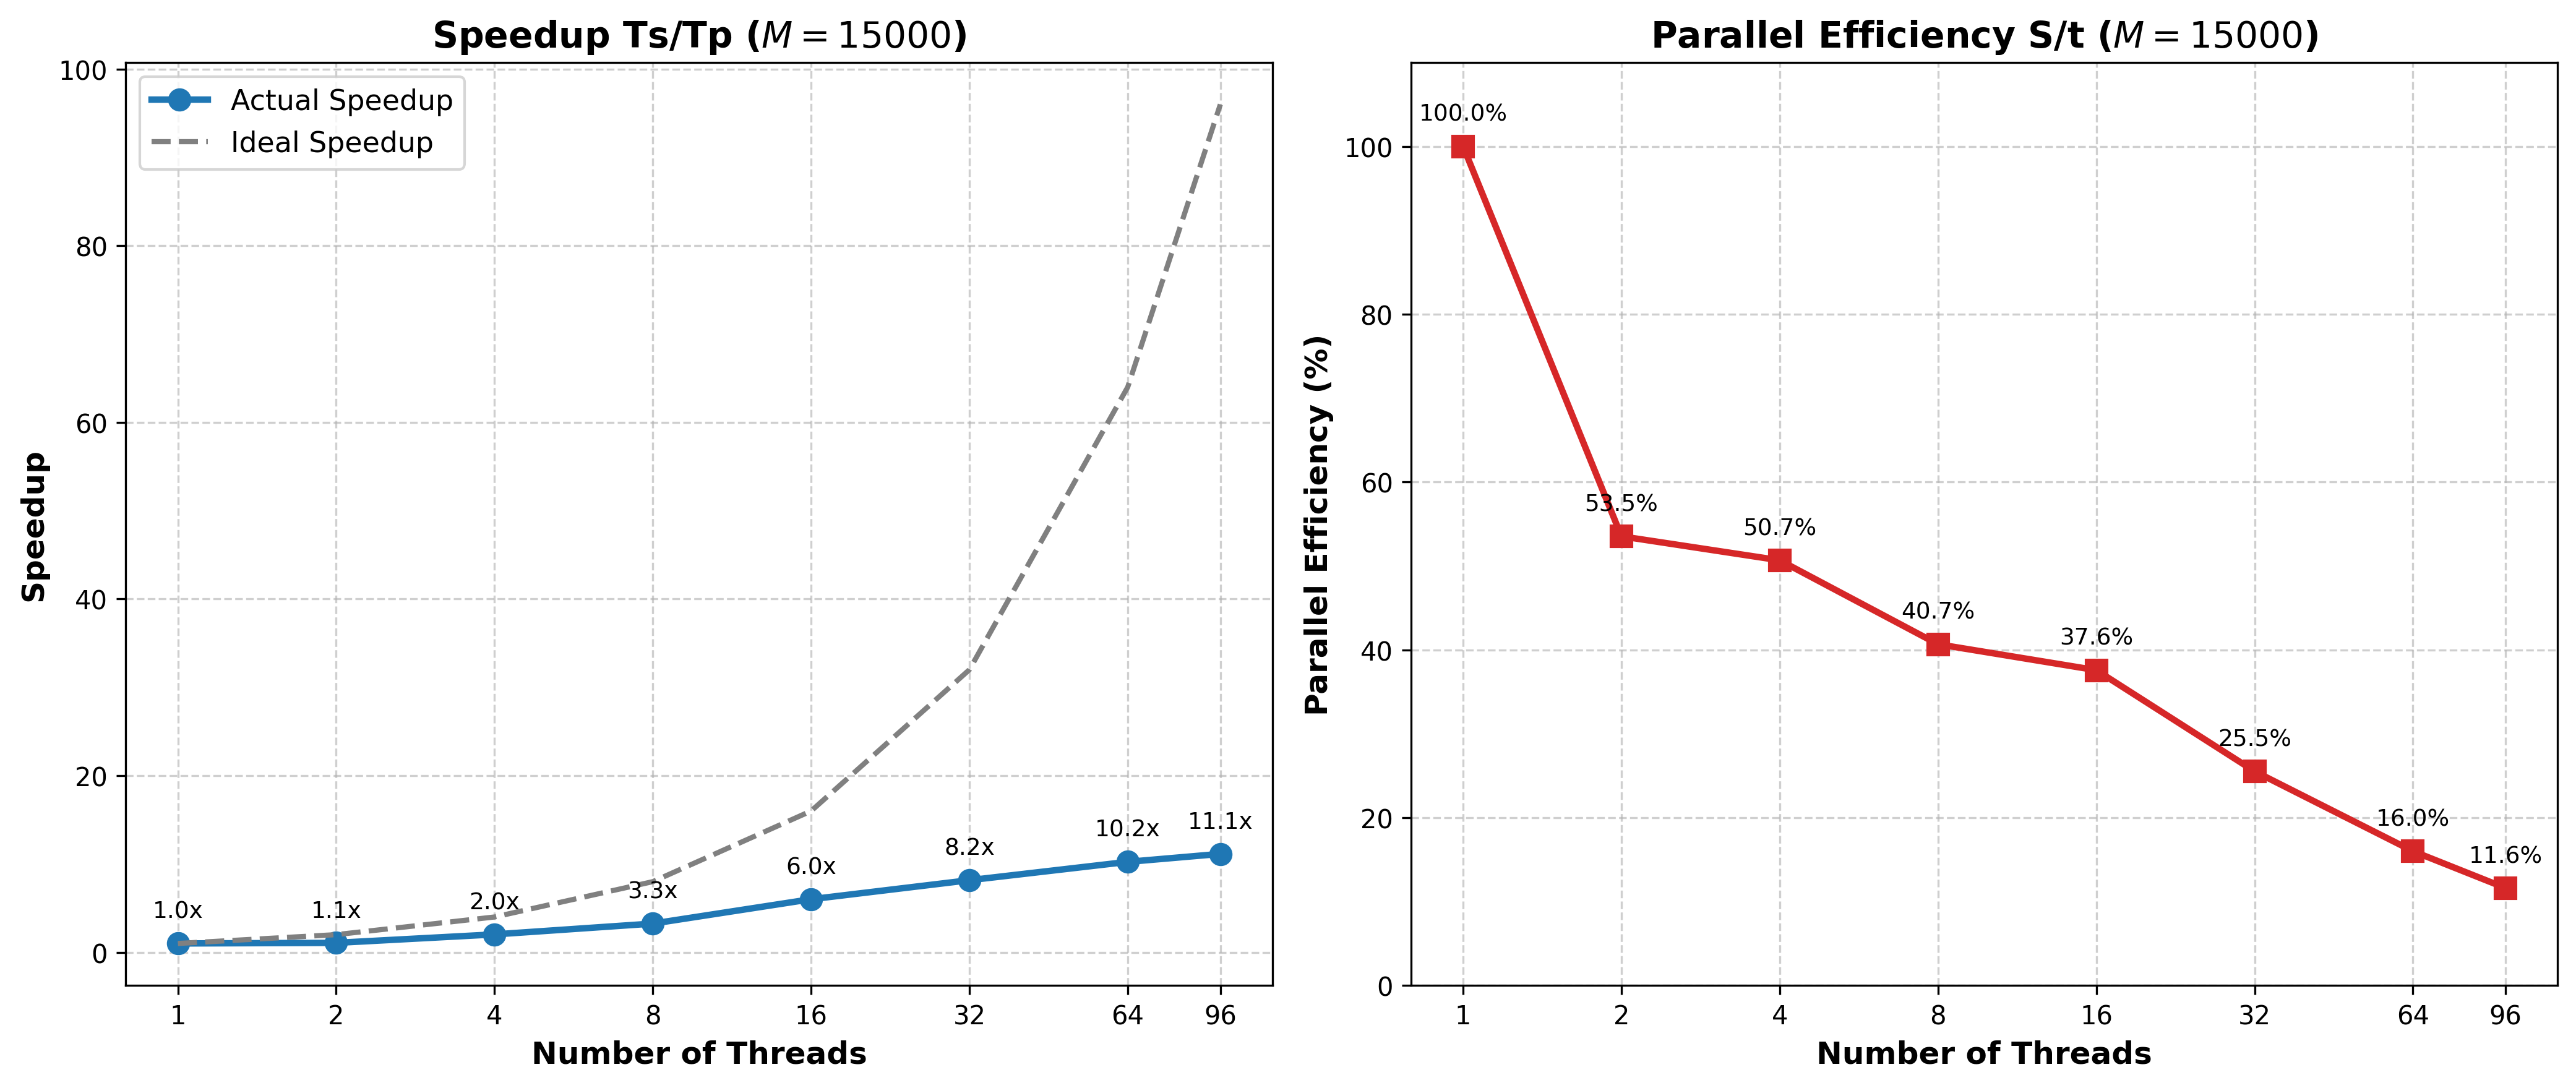
\includegraphics[width=0.5\textwidth]{../assignment_1/plots/scaling.png}
    \caption{Speedup and parallel efficiency with varying number of threads.}
    \label{fig:speedup}
\end{figure}
We then tested the program with a fixed workload size of $M=15000$ varying the number of threads and collected the \textbf{Speedup} and \textbf{Parallel Efficiency} (Speedup/Number of threads) parameters.
Figure~\ref{fig:speedup} shows two distinct regimes. For $P \leq 32$, all
threads run on independent physical cores; the efficiency loss
is explained by the OpenMP barriers cost, which
grows with team size. For $t=64$ and $t=96$, thread count exceeds the
number of physical cores (48), so Hyper-Threading is used from that point onward.

We repeated the same test with the I/O operations disabled, so that the
program only computes the matrix updates \cite{output_noio_sweep}.
Finally, we also replaced \texttt{schedule(guided)} with
\texttt{schedule(static)} in both the initialization and the stencil
loop, to restore the NUMA alignment mentioned earlier \cite{output_noio_static_sweep}. Once thread count
exceeds 24, work is necessarily split across both sockets, and accesses
to memory owned by the other socket incur the added latency of the
inter-socket interconnect.

\begin{figure}[h]
    \centering
    \begin{subfigure}[b]{0.47\textwidth}
        \centering
        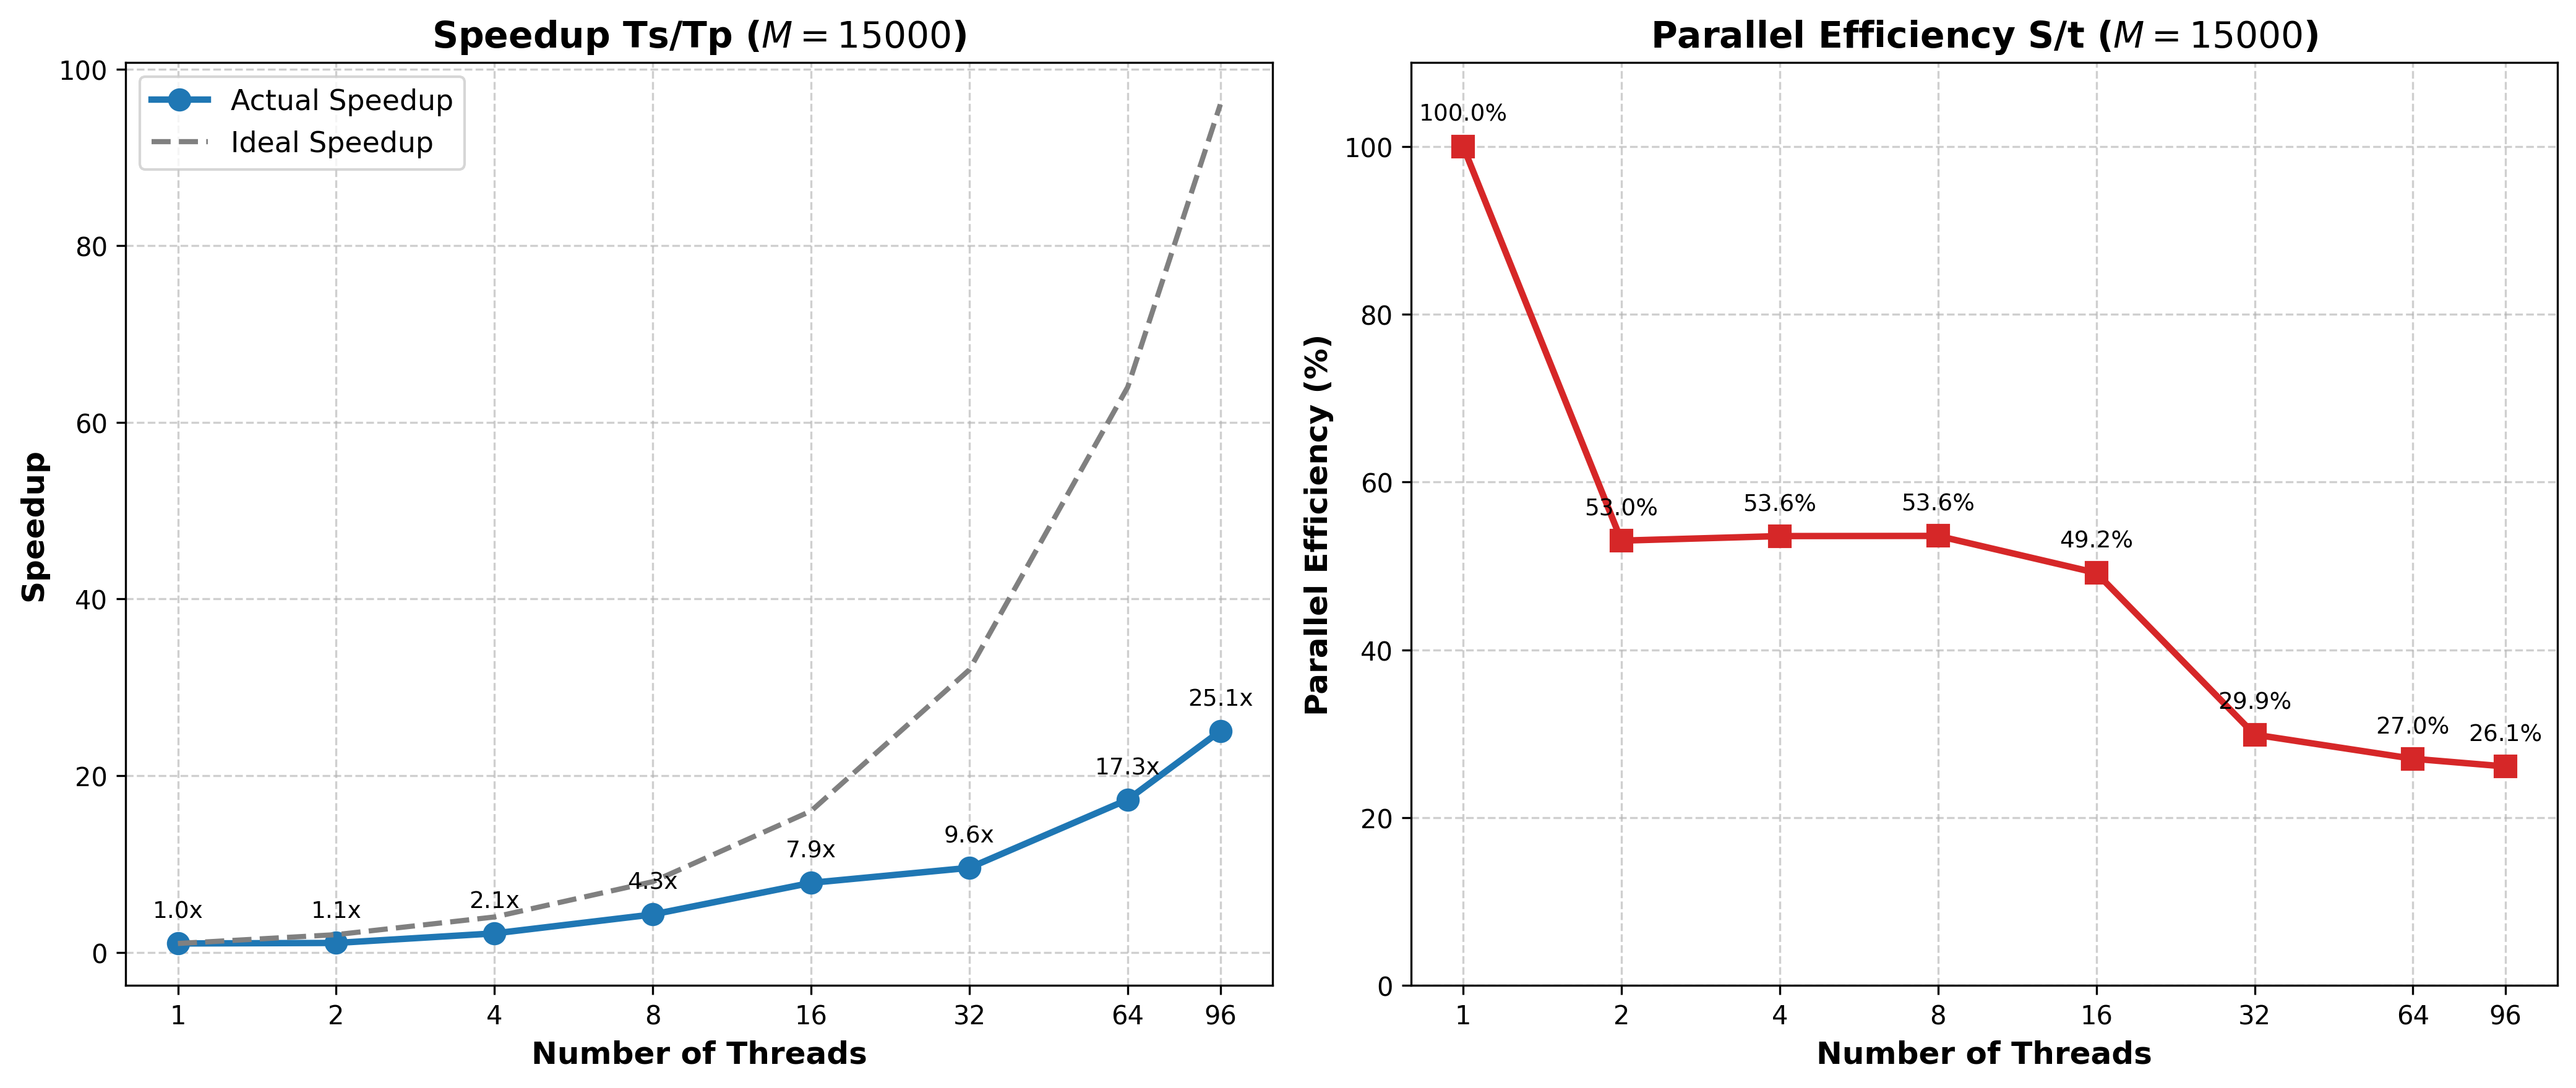
\includegraphics[width=\textwidth]{../assignment_1/plots/scaling_noio.png}
        \caption{\texttt{schedule(guided)}}
        \label{fig:speedup_noio}
    \end{subfigure}
    \hfill
    \begin{subfigure}[b]{0.47\textwidth}
        \centering
        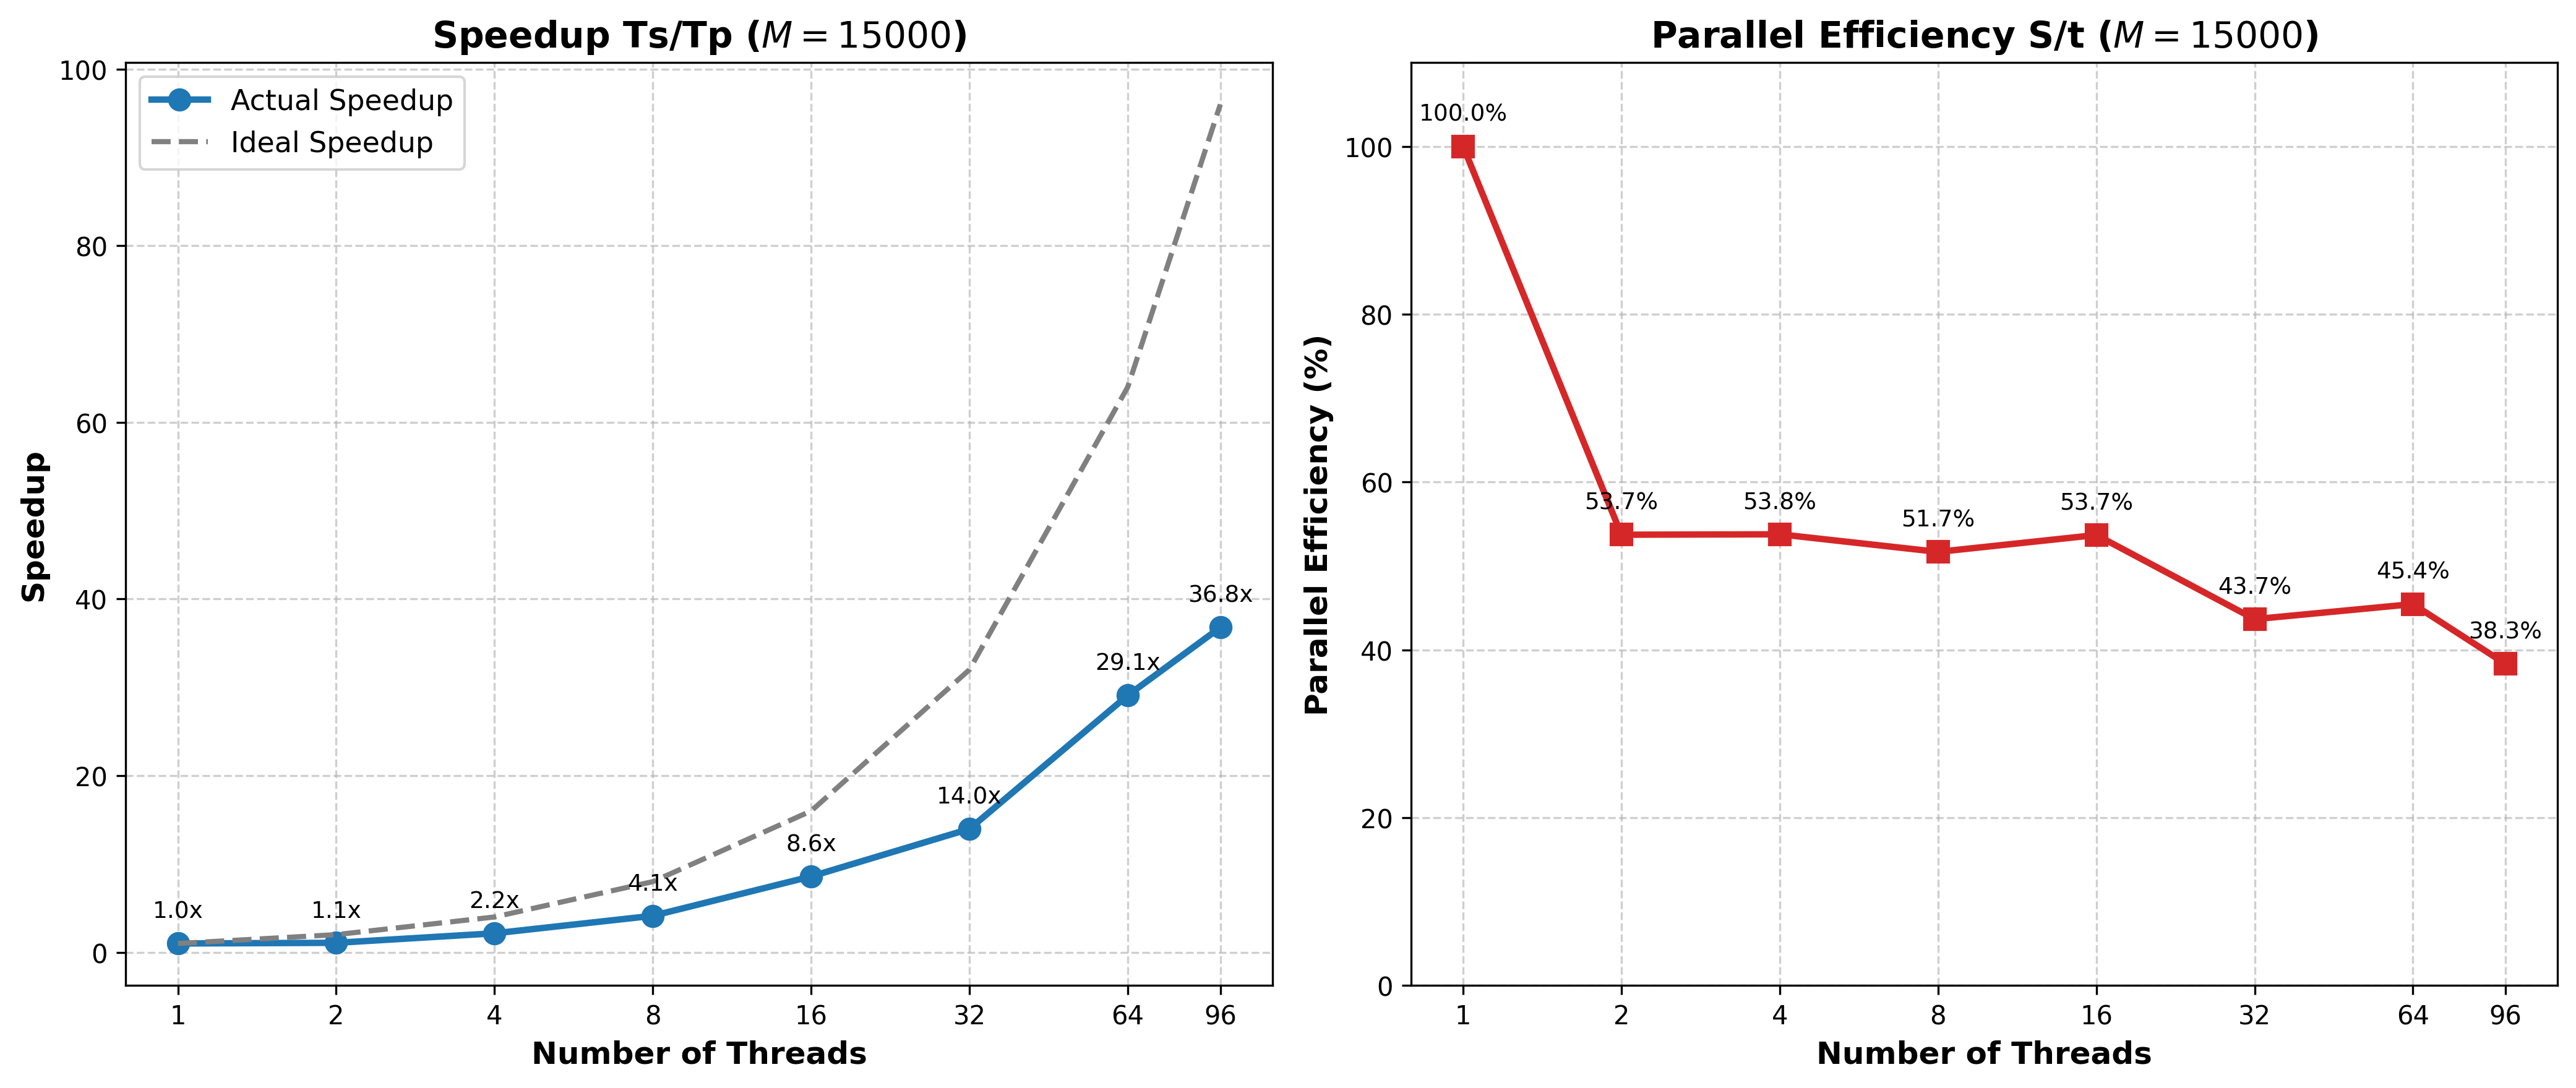
\includegraphics[width=\textwidth]{../assignment_1/plots/scaling_noio_static.png}
        \caption{\texttt{schedule(static)}}
        \label{fig:speedup_noio_static}
    \end{subfigure}
    \caption{Speedup and parallel efficiency with varying number of threads, I/O disabled.}
    \label{fig:speedup_noio_combined}
\end{figure}

As Figure~\ref{fig:speedup_noio} shows, both metrics improve
significantly: at $t=96$ speedup more than doubles, from $11.1\times$ to
$25.1\times$, and parallel efficiency grows from 11.6\% to 26.1\%. This
confirms that a substantial share of the overhead seen in the full
version came from the I/O operations and their associated
synchronization barriers, rather than from the stencil computation
itself.

As shown in Figure~\ref{fig:speedup_noio_static}, the static schedule
substantially mitigates this effect: the efficiency drop between $t=16$
and $t=32$ (the exact point where the 24-core NUMA boundary is crossed) is roughly halved (from $-19.3$ to $-10.0$ percentage points
relative to \texttt{guided}), and efficiency remains markedly higher at
$t=32$ (43.7\% vs. 29.9\%), $t=64$ (45.4\% vs. 27.0\%, a 68\% relative
gain) and $t=96$ (38.3\% vs. 26.1\%), with speedup at $t=96$ rising from
$25.1\times$ to $36.8\times$. This is consistent with the static schedule
preserving the same thread-to-row mapping established during
initialization, which keeps most memory accesses local to each thread's
own socket even as the workload spans both NUMA domains.
